% Options for packages loaded elsewhere
\PassOptionsToPackage{unicode}{hyperref}
\PassOptionsToPackage{hyphens}{url}
%
\documentclass[
]{book}
\usepackage{amsmath,amssymb}
\usepackage{lmodern}
\usepackage{iftex}
\ifPDFTeX
  \usepackage[T1]{fontenc}
  \usepackage[utf8]{inputenc}
  \usepackage{textcomp} % provide euro and other symbols
\else % if luatex or xetex
  \usepackage{unicode-math}
  \defaultfontfeatures{Scale=MatchLowercase}
  \defaultfontfeatures[\rmfamily]{Ligatures=TeX,Scale=1}
\fi
% Use upquote if available, for straight quotes in verbatim environments
\IfFileExists{upquote.sty}{\usepackage{upquote}}{}
\IfFileExists{microtype.sty}{% use microtype if available
  \usepackage[]{microtype}
  \UseMicrotypeSet[protrusion]{basicmath} % disable protrusion for tt fonts
}{}
\makeatletter
\@ifundefined{KOMAClassName}{% if non-KOMA class
  \IfFileExists{parskip.sty}{%
    \usepackage{parskip}
  }{% else
    \setlength{\parindent}{0pt}
    \setlength{\parskip}{6pt plus 2pt minus 1pt}}
}{% if KOMA class
  \KOMAoptions{parskip=half}}
\makeatother
\usepackage{xcolor}
\IfFileExists{xurl.sty}{\usepackage{xurl}}{} % add URL line breaks if available
\IfFileExists{bookmark.sty}{\usepackage{bookmark}}{\usepackage{hyperref}}
\hypersetup{
  pdftitle={Introduction to Statistics},
  pdfauthor={Aaron McMurray},
  hidelinks,
  pdfcreator={LaTeX via pandoc}}
\urlstyle{same} % disable monospaced font for URLs
\usepackage{longtable,booktabs,array}
\usepackage{calc} % for calculating minipage widths
% Correct order of tables after \paragraph or \subparagraph
\usepackage{etoolbox}
\makeatletter
\patchcmd\longtable{\par}{\if@noskipsec\mbox{}\fi\par}{}{}
\makeatother
% Allow footnotes in longtable head/foot
\IfFileExists{footnotehyper.sty}{\usepackage{footnotehyper}}{\usepackage{footnote}}
\makesavenoteenv{longtable}
\usepackage{graphicx}
\makeatletter
\def\maxwidth{\ifdim\Gin@nat@width>\linewidth\linewidth\else\Gin@nat@width\fi}
\def\maxheight{\ifdim\Gin@nat@height>\textheight\textheight\else\Gin@nat@height\fi}
\makeatother
% Scale images if necessary, so that they will not overflow the page
% margins by default, and it is still possible to overwrite the defaults
% using explicit options in \includegraphics[width, height, ...]{}
\setkeys{Gin}{width=\maxwidth,height=\maxheight,keepaspectratio}
% Set default figure placement to htbp
\makeatletter
\def\fps@figure{htbp}
\makeatother
\setlength{\emergencystretch}{3em} % prevent overfull lines
\providecommand{\tightlist}{%
  \setlength{\itemsep}{0pt}\setlength{\parskip}{0pt}}
\setcounter{secnumdepth}{5}
\usepackage{booktabs}
\ifLuaTeX
  \usepackage{selnolig}  % disable illegal ligatures
\fi
\usepackage[]{natbib}
\bibliographystyle{apalike}

\title{Introduction to Statistics}
\author{Aaron McMurray}
\date{2022-06-09}

\begin{document}
\maketitle

{
\setcounter{tocdepth}{1}
\tableofcontents
}
\hypertarget{Introduction-to-Statistics}{%
\chapter*{Introduction to Statistics}\label{Introduction-to-Statistics}}
\addcontentsline{toc}{chapter}{Introduction to Statistics}

\textbf{Overview}

This resource is intended to provide an introduction to the basics of statistics.

\textbf{Contents}

\begin{itemize}
\tightlist
\item
  Introduction
\item
  Data Types and Levels of Measurement
\item
  Describing Data
\item
  Comparing Data
\item
  Data Visualisation
\item
  Correlation
\item
  Sampling
\item
  Confidence Intervals
\item
  Hypothesis Testing
\item
  Statistical Significance
\item
  Odds against Chance Fallacy
\item
  Statistical Significance Verses Importance
\end{itemize}

\hypertarget{intro}{%
\chapter{Introduction}\label{intro}}

\hypertarget{what-is-statistics}{%
\section{What is Statistics?}\label{what-is-statistics}}

Statistics is all about the collection, organization, analysis, interpretation and presentation of data. Statistics is used everywhere from opinion polling in politics to predicting the prices of assets. There are two main branches of statistics: descriptive statistics and inferential statistics.

\hypertarget{descriptive-statistics}{%
\section{Descriptive Statistics}\label{descriptive-statistics}}

Descriptive statistics describes or summarises data that have been collected. Measures of central tendency such as (mean, median and the mode) and measures of dispersion (range, interquartile range and standard deviation) are the most important tools.

\hypertarget{inferential-statistics}{%
\section{Inferential Statistics}\label{inferential-statistics}}

Inferential statistical is used to make prediction about a population using information gathered about a sample. Inferential statistics involves hypothesis testing and regression analysis.

\hypertarget{data-types-and-levels-of-measurement}{%
\chapter{Data Types and Levels of Measurement}\label{data-types-and-levels-of-measurement}}

\hypertarget{types-of-data}{%
\section{Types of Data}\label{types-of-data}}

Data can be broadly categorised as \textbf{qualitative} (data relating to qualities or characteristics) or quantitative (numerical data relating to sizes or quantities of things).

We can further categorise \textbf{quantitative} data as being continuous or discrete.

\textbf{Discrete} data involves whole numbers that can't be divided because of what they represent (number of people in a class, number of cars owned). The number of people in a class cannot be 10.5 or 3.14. It must be a whole number because people are not divisible.

\textbf{Continuous} data can be divided and measured to some number of decimal places (height, weight, speed in miles per hour). A person's height can be any number (provided it lies within the range of possible human heights) and can be reported to any number of decimal places (150cm or 150.1cm or 150.12cm) depending on how accurate the measurement tool is.

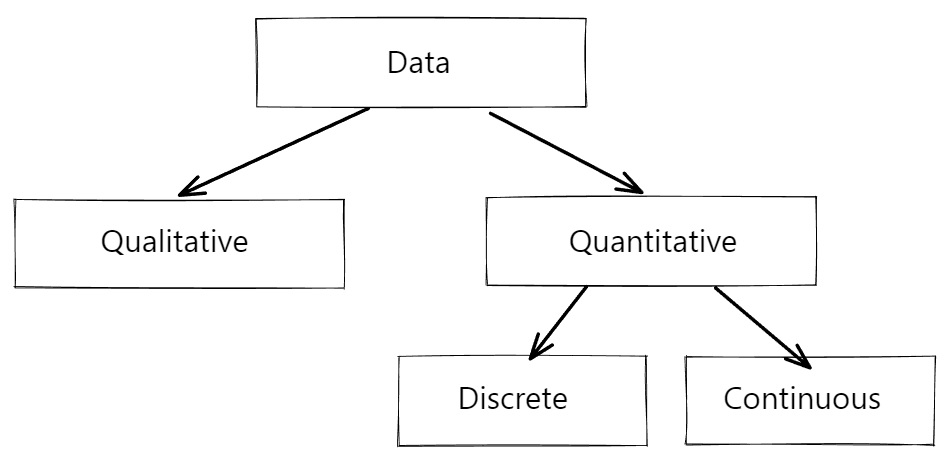
\includegraphics{data.jpg}
There are also different \textbf{levels of measurement}.

\hypertarget{levels-of-measurement}{%
\section{Levels of Measurement}\label{levels-of-measurement}}

The levels of measurement describe how precisely variables are recorded. The different levels of measurement limit which statistics can be used to summarise data and which inferential statistics can be performed. These levels are:

\begin{itemize}
\tightlist
\item
  Nominal
\item
  Ordinal
\item
  Interval
\item
  Ratio
\end{itemize}

\hypertarget{nominal}{%
\subsection{Nominal}\label{nominal}}

\textbf{Nominal data} is a type of data that is used to label variables. It can be categorised but not ranked (eye colour and gender for instance). The values grouped into these categories have no meaningful order. It is not possible to form a meaningful hierarchy of gender or eye colour.

\begin{figure}

{\centering 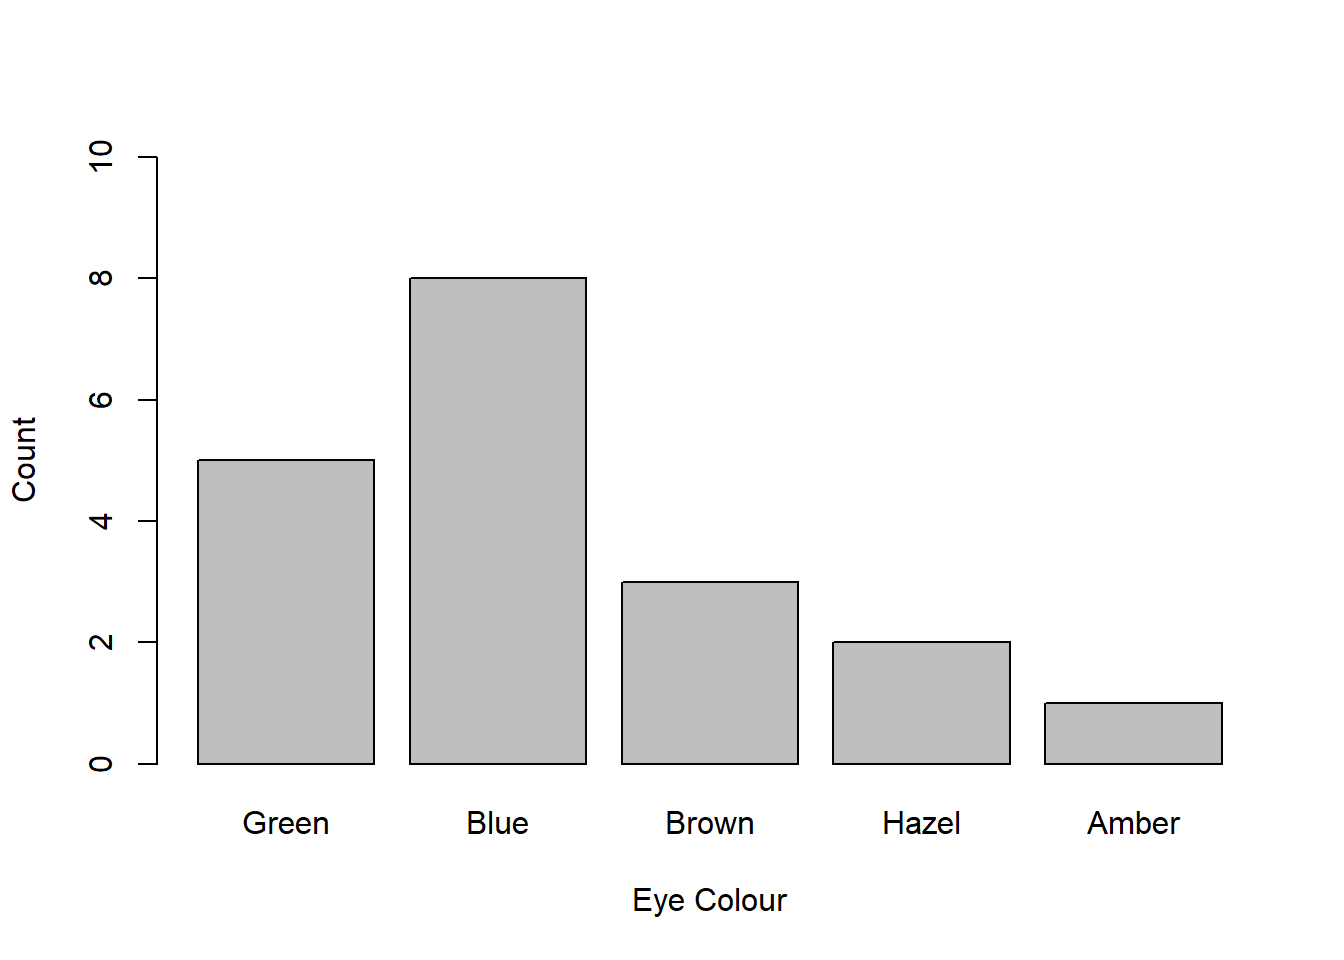
\includegraphics{Bookdown_files/figure-latex/chunk-label-1} 

}

\caption{Eye colour is an example of nominal data.}\label{fig:chunk-label}
\end{figure}

The only measure of central tendency used with nominal data is the mode.

\hypertarget{ordinal}{%
\subsection{Ordinal}\label{ordinal}}

\textbf{Ordinal data} is another type of \textbf{qualitative data} that groups variables into descriptive categories. The categories used for ordinal data are ordered in some kind of hierarchical scale although the distance between those categories may be uneven or even unknown.

\begin{figure}

{\centering 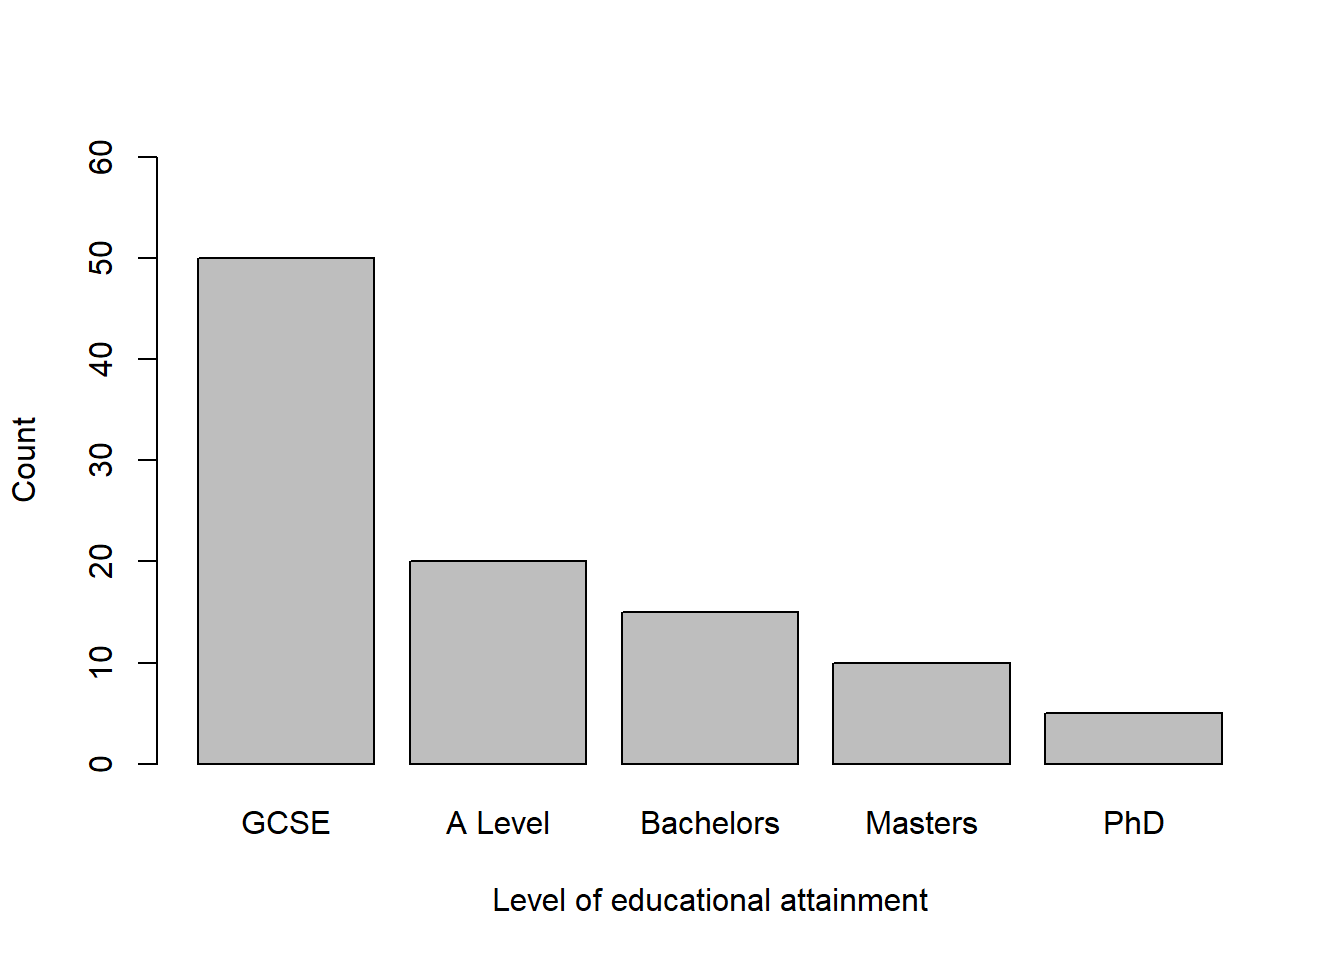
\includegraphics{Bookdown_files/figure-latex/unnamed-chunk-1-1} 

}

\caption{The highest level of educational attainment has a heirarchical scale but the distance between categories is unclear.}\label{fig:unnamed-chunk-1}
\end{figure}

Ordinal variables often include ratings about opinions that can be categorised (strongly agree, agree, don't know, disagree, strongly disagree).

The descriptive statistics which can be used with ordinal data are the mode and the median.

Ordinal data can also be described with a measure of dispersion, namely, range.

\hypertarget{interval}{%
\subsection{Interval}\label{interval}}

\textbf{Interval data} is a type of quantitative data that groups variables into categories. Values can be ordered and separated using an equal measure of distance.

An example of interval level data is temperature data recorded in Celsius or Fahrenheit. The values on either scale are ordered and separated using an equal measure of distance (the distances between notches on a thermometer are always equally spaced).

\begin{figure}

{\centering 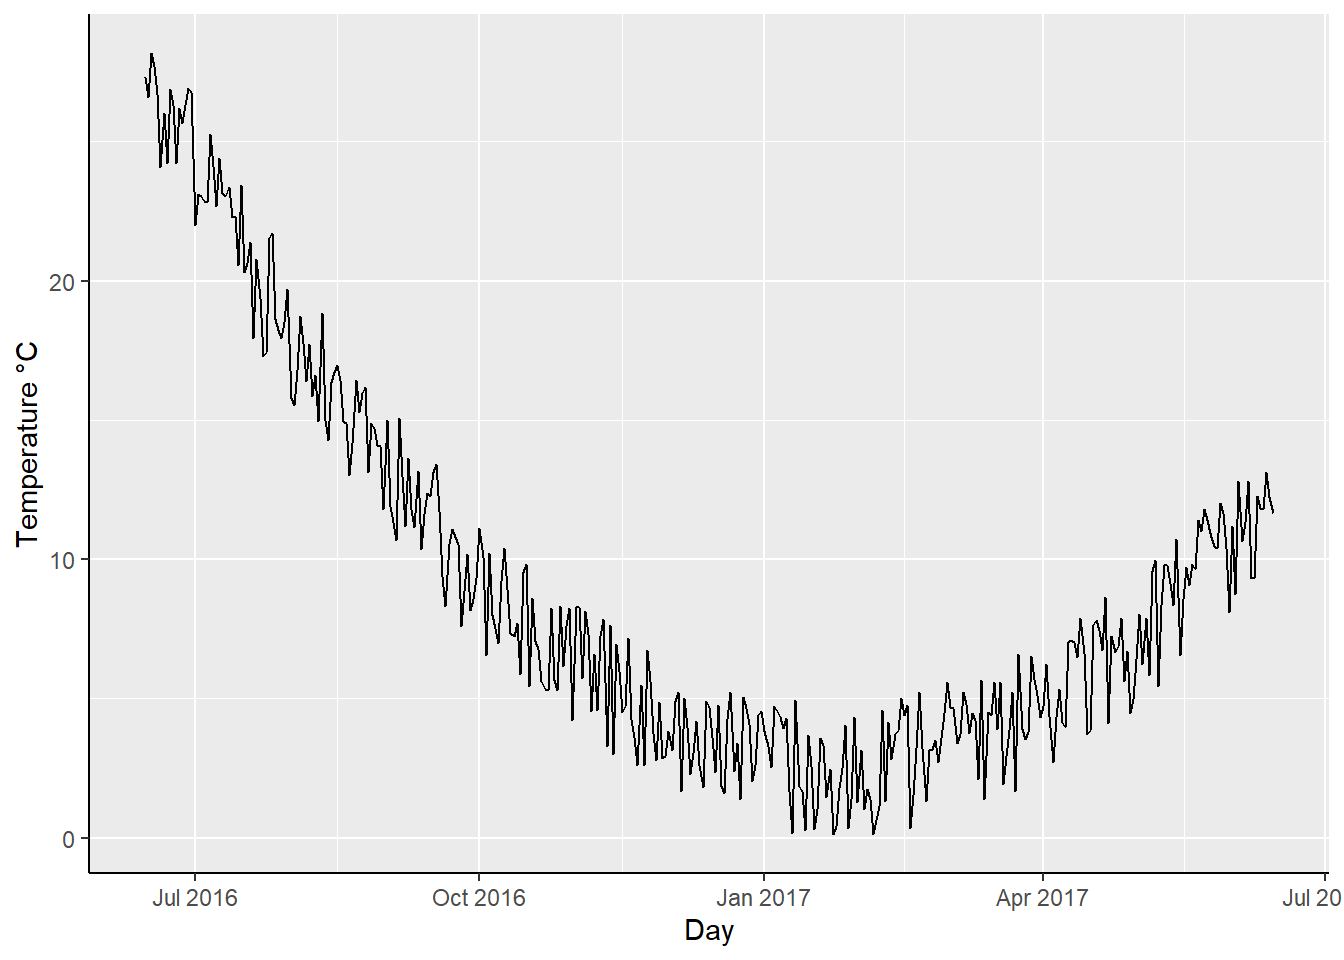
\includegraphics{Bookdown_files/figure-latex/unnamed-chunk-2-1} 

}

\caption{Temperature in Celsius is interval data. The values are ordered and separated by an equal interval. The distance between 0°C and 1°C is the same as the distance between 2°C and 3°C.}\label{fig:unnamed-chunk-2}
\end{figure}

Mathematical operations can be carried out on this type of data, for instance, subtracting one value from another to find the difference. Interval data lacks a \textbf{true zero}.

True zero indicates a lack of whatever is being measured. The Celsius scale doesn't qualify as having a true zero since the zero point in a thermometer is arbitrary. When the Celsius scale was first created by Anders Celsius 0°C was selected to match the boiling point of water and a value of 100 °C was the freezing point of water. The scale was later reversed. Thermometers measure heat and at 0°C there is still heat, maybe not a great deal of it but heat is still measurable meaning 0°C is not a true zero. The thermodynamic Kelvin Scale has a true zero - where particles have no motion and can become no colder (there is a true absence of heat).

A range of descriptive statistics can be used to describe interval data. The measures of central tendency applicable to interval data are the \textbf{mode, median} and the \textbf{mean}. The measures of dispersion applicable to interval data are the \textbf{range, standard deviation} and the \textbf{variance}.

\hypertarget{ratio}{%
\subsection{Ratio}\label{ratio}}

\textbf{Ratio data} is a form of quantitative data. It measures variables on a continuous scale with an equal distance between adjacent values (weight, height). Ratio data has a true zero. Ratio data is the most complex of the four data types.

\begin{figure}

{\centering 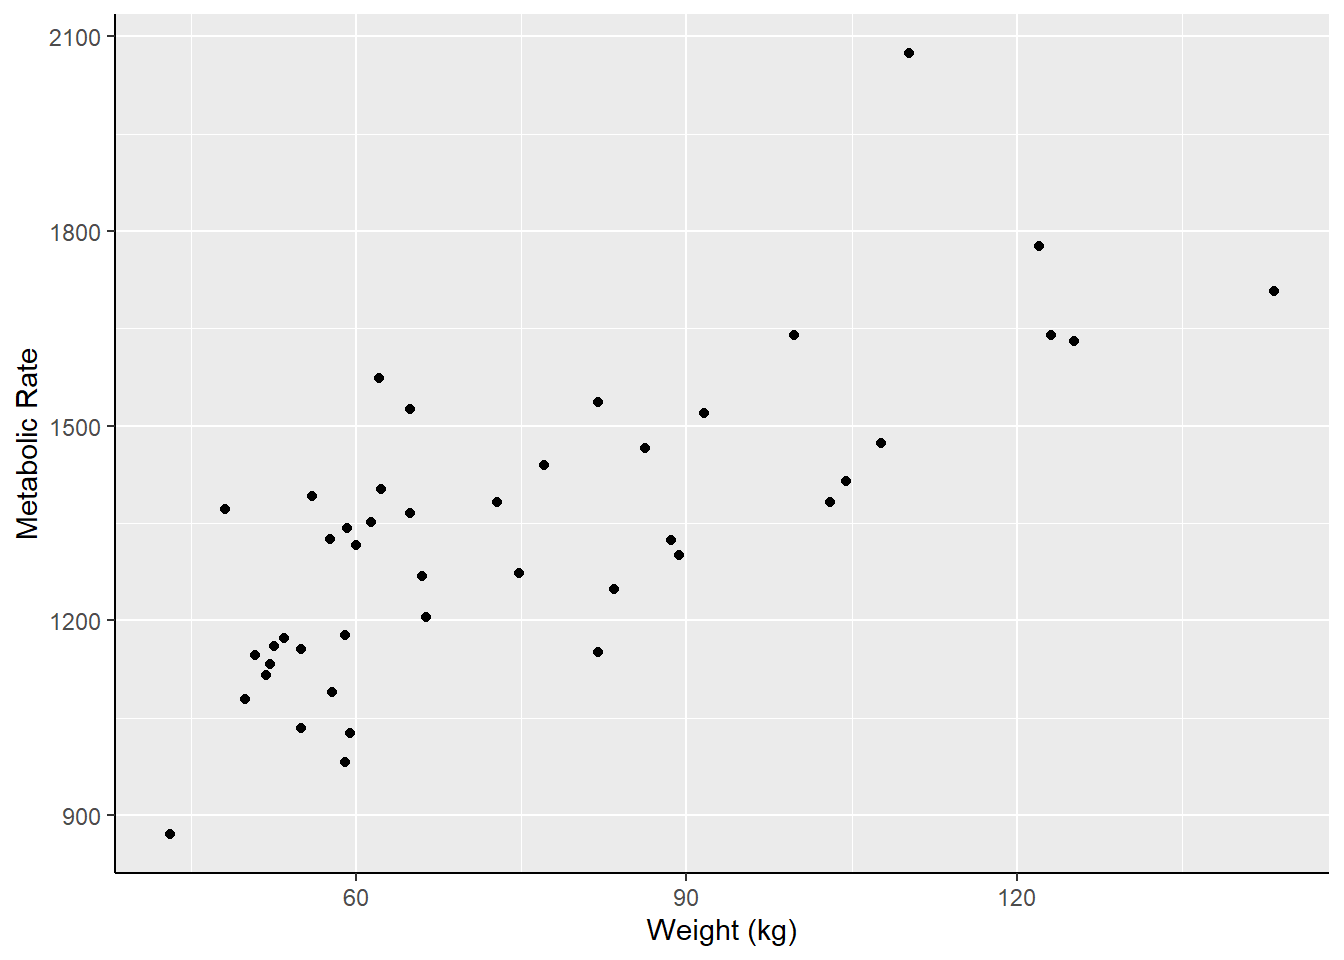
\includegraphics{Bookdown_files/figure-latex/unnamed-chunk-3-1} 

}

\caption{The scatterplot above shows metabolic rate plotted against body weight (kg). These are examples of ratio data.}\label{fig:unnamed-chunk-3}
\end{figure}

Ratio data can be analysed with descriptive statistics including the \textbf{mode, median} and \textbf{mean}. \textbf{Range, standard deviation, variance} and the \textbf{coefficient of variation} can all be used to describe the dispersion of ratio data.

\hypertarget{quiz}{%
\chapter{Quiz}\label{quiz}}

Take the \href{https://view.genial.ly/62867083cd8fd700184ca06f/presentation-quiz}{Levels of Measurement Quiz} below to test how well you understand the levels of measurement.

\begin{center}\includegraphics[width=1\linewidth]{quizpic} \end{center}

\hypertarget{describing-data}{%
\chapter{Describing Data}\label{describing-data}}

\hypertarget{frequency}{%
\section{Frequency}\label{frequency}}

The \textbf{frequency} of an observation is the number of times it occurs or is recorded.A frequency table, like the one shown below detailing exam grades, is a commonly used method of depicting frequency.

\begin{longtable}[]{@{}rr@{}}
\caption{\label{tab:table2}Frequency Table}\tabularnewline
\toprule
Grade & Frequency \\
\midrule
\endfirsthead
\toprule
Grade & Frequency \\
\midrule
\endhead
A & 15 \\
B & 20 \\
C & 25 \\
D & 21 \\
E & 14 \\
\bottomrule
\end{longtable}

The total of all frequencies so far in a frequency distribution is the \textbf{cumulative frequency}. It is the `running total' of frequencies.

\begin{longtable}[]{@{}rrr@{}}
\caption{\label{tab:table3}Cumulative Frequency Table}\tabularnewline
\toprule
Grade & Frequency & Cumulative Frequency \\
\midrule
\endfirsthead
\toprule
Grade & Frequency & Cumulative Frequency \\
\midrule
\endhead
A & 15 & 15 \\
B & 20 & 35 \\
C & 25 & 60 \\
D & 21 & 81 \\
E & 14 & 95 \\
\bottomrule
\end{longtable}

The \textbf{relative frequency} is the ratio of the category frequency to the total number of outcomes. For grade A, the relative frequency is:

\[ \frac{15}{15+20+25+21+14}=0.16. \]

The table can be extended to include the relative frequency.

\begin{longtable}[]{@{}rrr@{}}
\caption{\label{tab:table4}Relative Frequency Table}\tabularnewline
\toprule
Grade & Frequency & Relative Frequency \\
\midrule
\endfirsthead
\toprule
Grade & Frequency & Relative Frequency \\
\midrule
\endhead
A & 15 & 0.16 \\
B & 20 & 0.21 \\
C & 25 & 0.26 \\
D & 21 & 0.22 \\
E & 14 & 0.15 \\
\bottomrule
\end{longtable}

The \textbf{relative frequency} can be reported as a percentage by multiplying the values by 100\%. For grade A, the relative frequency reported as a percentage is: 100\% x 0.16 = 16\%.

\hypertarget{measures-of-central-tendency}{%
\section{Measures of Central Tendency}\label{measures-of-central-tendency}}

Measures of central tendency help find the middle, or the average, of a data set.The measures of central tendency are the mean, median and mode.

\hypertarget{mean}{%
\subsection{Mean}\label{mean}}

The mean is the sum of the recorded values divided by the number of values recorded.

\hypertarget{example}{%
\subsubsection{Example}\label{example}}

Find the mean of this list of numbers:

\[ 2, 3, 3, 4, 20.\]
\[ \textrm{Mean} = \frac{\textrm{Sum of recorded values}}{\textrm{Number of values recorded}},\]
\[ \textrm{Mean} = \frac{\textrm{2 + 3 + 3 + 4 + 20}}{\textrm{5}},\]
\[ \textrm{Mean} = \frac{\textrm{32}}{\textrm{5}},\]

\[ \textrm{Mean} = 6.4.\]

\hypertarget{median}{%
\subsection{Median}\label{median}}

The \textbf{median} is the middle number in a sorted, ascending or descending, list of values.

If there are an odd number of values the median is simply the middle value.

For an even number of values there will be two values in the center. Those values are summed and divided by two.

The median is sometimes used as opposed to the mean when there are outliers that might skew the average of the values.

\hypertarget{example-1}{%
\subsubsection{Example}\label{example-1}}

Find the median of this list of numbers:

\[ 2, 3, 3, 4, 20.\]

There are 5 values listed in ascending order and the middle value is the third value in the list so the median is 3.

Note: In the previous example the mean was 6.4. It was skewed by the outlier (20). The median remains closer to what might be considered to be the middle of the data set.

\hypertarget{example-2}{%
\subsubsection{Example}\label{example-2}}

Find the median of this list of numbers:

\[ 3, 5, 4, 4, 2, 8, 7, 1.\]

The list should be sorted:

\[ 1, 2, 3, 4, 4, 5, 7, 8. \]

There are an even number of values so there will be two middle values. The middle values are 4 and 4. Sum them and divide by two to get the median: 4.

\hypertarget{mode}{%
\subsection{Mode}\label{mode}}

The mode of a set of data values is the value that appears most often. It is the value that is most likely to be sampled. There can be multiple modes or no modes.

\hypertarget{example-3}{%
\subsubsection{Example}\label{example-3}}

Find the mode of this list of numbers:

\[ 1, 2, 2, 2, 3, 3, 4.\]

A simple way to find the mode is to make a frequency table with the unique values on the left hand side and their frequency on the right hand side. We can tally up how many times each number occurs. Whichever has the greatest frequency is our mode.

\begin{longtable}[]{@{}rr@{}}
\caption{\label{tab:table5}Frequency Table}\tabularnewline
\toprule
Value & Frequency \\
\midrule
\endfirsthead
\toprule
Value & Frequency \\
\midrule
\endhead
1 & 1 \\
2 & 3 \\
3 & 2 \\
4 & 1 \\
\bottomrule
\end{longtable}

The mode is 2.

\hypertarget{example-4}{%
\subsubsection{Example}\label{example-4}}

Find the mode of this list of numbers:

\[ 7, 3, 5, 3, 4, 3, 5, 6, 8, 5.\]

\begin{longtable}[]{@{}rr@{}}
\caption{\label{tab:table6}Frequency Table}\tabularnewline
\toprule
Value & Frequency \\
\midrule
\endfirsthead
\toprule
Value & Frequency \\
\midrule
\endhead
3 & 3 \\
4 & 1 \\
5 & 3 \\
6 & 1 \\
7 & 1 \\
8 & 1 \\
\bottomrule
\end{longtable}

This is \textbf{bimodal}, it has two modes, 3 and 5.

\hypertarget{example-5}{%
\subsubsection{Example}\label{example-5}}

Find the mode of this list of numbers:

\[ 1, 2, 3, 4, 5, 6.\]

\begin{longtable}[]{@{}rr@{}}
\caption{\label{tab:table7}Frequency Table}\tabularnewline
\toprule
Value & Frequency \\
\midrule
\endfirsthead
\toprule
Value & Frequency \\
\midrule
\endhead
1 & 1 \\
2 & 1 \\
3 & 1 \\
4 & 1 \\
5 & 1 \\
6 & 1 \\
\bottomrule
\end{longtable}

Every value is unique and occurs only once so this data has no mode.

\hypertarget{using-excel}{%
\section{Using Excel}\label{using-excel}}

It is useful to calculate descriptive statistics by hand for understanding but for larger data sets it is not always possible to arrange data and perform calculations by hand.

Excel has a number of functions designed to perform descriptive statistics.

\textbf{Frequency}

=FREQUENCY(start:end,bins\_array)

The frequency() function will return a frequency table describing your data. It takes two arguments, the first being the array of values and the second being an array describing the upper boundary of the bins used.

\textbf{Average}

=AVERAGE(start:end)

The mean is calculated using the average() function. There are several other functions relating to means: geomean(), harmean() and trimmean(). Take care not to use these as they are quite different from calculating the mean that has been described here.

\textbf{Median}

=MEDIAN(start:end)

The median is calculated using the median() function.

\textbf{Mode}

=MODE.SNGL(start:end)

=MODE.MULT(start:end)

There are several functions for calculating the mode: mode(), mode.sngl() and mode.mult().
mode() was used in Excel 2007 and may still appear as an option in some versions of Excel.
mode.sngl() will return one mode and mode.mult() will return multiple modes (if there are multiple modes).

Neither mode() nor mode.sngl() will warn you if there are multiple modes so mode.mult() is usually the safest option.

\hypertarget{example-6}{%
\subsection{Example}\label{example-6}}

In the example below, the variable name is in cell A1 and the values are in cells A2 to A18. To calculate the average, type ``=AVERAGE(A2:A18)'' in another cell. It doesn't matter which cell but in this example A19 has been used. Press enter to return the value.

\begin{figure}
\centering
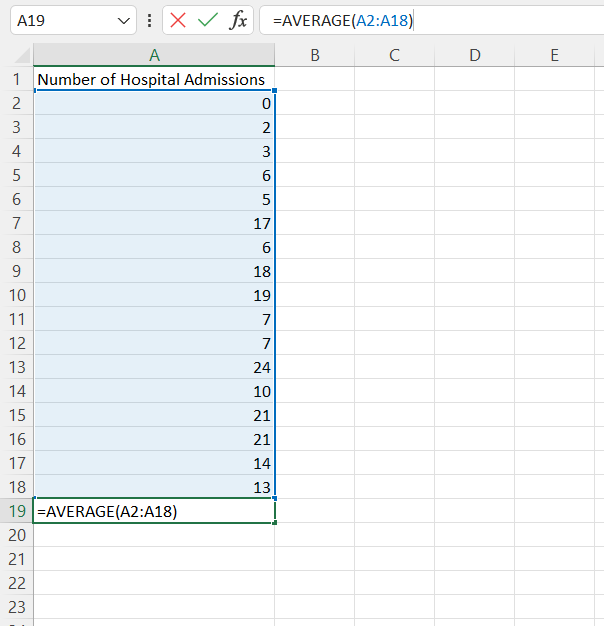
\includegraphics{Excelimage.png}
\caption{Screen shot showing excel spreadsheet with a list of values and the average being calculated using the average() function.}
\end{figure}

\hypertarget{measures-of-dispersion}{%
\section{Measures of Dispersion}\label{measures-of-dispersion}}

\textbf{Dispersion} (or variability) describes how far apart data points lie from each other and the center of a distribution. The \textbf{range, interquartile range, variance} and \textbf{standard deviation} are all measures of dispersion and they describe how far apart data points lie from one another and the center of a distribution.

\hypertarget{range}{%
\subsection{Range}\label{range}}

The range is the difference between the highest and lowest values and is calculated by subtracting the minimum value from the maximum value.

\hypertarget{example-7}{%
\subsubsection{Example}\label{example-7}}

Calculate the range for the following set of numbers:

\[ 23, 42, 75, 19, 74. \]
First, arrange the values in ascending order:

\[ 19, 23, 42, 74, 75. \]
The maximum value is 75 and the minimum is 19.

\[ \textrm{Range}= 75 - 19, \]
\[ \textrm{Range} = 56.\]

\hypertarget{interquartile-range}{%
\subsection{Interquartile Range}\label{interquartile-range}}

The \textbf{interquartile range} (IQR) describes the spread of the middle half of a distribution. How the interquartile range is calculated depends on whether there are an even or an odd number of values in a dataset.

For an even number of values the dataset in split half. The medians for the two new subsets of data are calculated. The positive difference of those medians is the interquartile range.
For an odd number of values either the inclusive or the exclusive method of finding the interquartile range must be used.

\begin{figure}
\centering
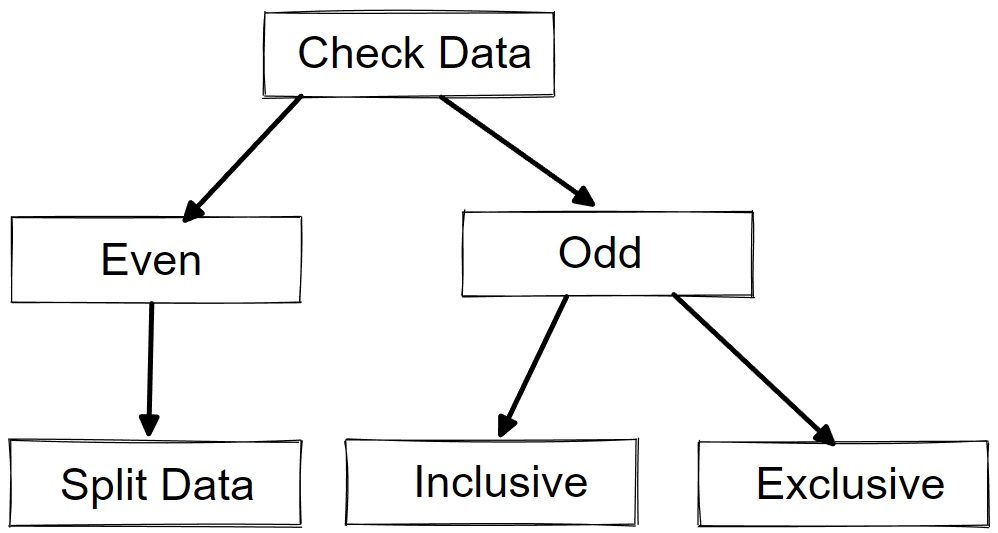
\includegraphics{iqrtree.jpg}
\caption{Tree diagram showing process of deciding how to calculate the IQR}
\end{figure}

The algorithm for the \textbf{exclusive method} is detailed below:

\begin{enumerate}
\def\labelenumi{\arabic{enumi}.}
\tightlist
\item
  Arrange the data in numeric order.
\item
  Remove the median and split the data about its center.
\item
  Find the medians of the two newly appended subsets of data.
\item
  Calculate the difference.
\end{enumerate}

The algorithm for the \textbf{inclusive method} is detailed below:

\begin{enumerate}
\def\labelenumi{\arabic{enumi}.}
\tightlist
\item
  Arrange the data in numeric order.
\item
  Remove the median and split the data about its center.
\item
  Append the two new subsets of data with the median.
\item
  Find the medians of the two newly appended subsets of data.
\item
  Calculate the difference.
\end{enumerate}

Click on the slides below to see some examples.

\begin{center}\includegraphics[width=1\linewidth]{quizpic} \end{center}

\hypertarget{variance-and-standard-deviation}{%
\subsection{Variance and Standard Deviation}\label{variance-and-standard-deviation}}

The standard deviation describes to what extent a set of numbers lie apart (their spread). It is the square root of variance which is also an indicator of the spread of values.

\textbf{Variance}

To calculate the variance:
1. Start by finding the mean of the values in the dataset.
2. Find the difference between each recorded value and the mean.
3. Square those differences.
4. Sum the squared differences.
5. Divide the sum by the number of values recorded for population variance or the sum of the number of values minus 1 for sample variance.

\textbf{Standard Deviation}

Taking square root of the variance corrects for the fact that all the differences were squared, resulting in the standard deviation.

The plot below shows three distributions of values, each with a mean of 30 but with different standard deviations. In statistics there is a rule called the empirical rule that states that 68\%, 95\%, and 99.7\% of the values lie within one, two, and three standard deviations of the mean, respectively.

\begin{center}\includegraphics[width=1\linewidth]{quizpic} \end{center}

\hypertarget{methods}{%
\chapter{Methods}\label{methods}}

We describe our methods in this chapter.

\hypertarget{final-words}{%
\chapter{Final Words}\label{final-words}}

We have finished a nice book.

  \bibliography{book.bib,packages.bib}

\end{document}
